% ============================================================
%  N.2.2  DepFiN CS2+CS3: PE Row and Column Sweeps
% ============================================================
\subsection{DepFiN: PE Row and Column Sweeps (CS2, CS3)}
\label{sec:cs2-cs3}

\subsubsection{Motivation}

The two spatial dimensions of the DepFiN PE array serve different
purposes: columns are mapped to the output width~$Q$ (determining the maximum output tile size available to be chosen), while rows are mapped to output channels~$Z$.
Adding PEs along one dimension therefore has a qualitatively different
effect from adding them along the other.
We select to explore three potential PEs configuration for activation dominant workloads, and four for weight dominant workloads.
CS2 and CS3 isolate these two effects by sweeping one dimension at a
time while keeping the other fixed.

\paragraph{CS2: Row Sweep.}
The number of PE rows is varied (8, 16, 32 for FSRCNN and MC-CNN;
16, 32, 64, 128 for VGG16 and ResNet18) while columns are fixed at
128.
More rows allow more output channels to be computed in parallel,
reducing the number of temporal iterations over~$Z$ and, consequently,
the number of times input activations are re-read from the Feature
Memory.

\paragraph{CS3: Column Sweep.}
The number of PE columns is varied (64, 128, 256 for FSRCNN and
MC-CNN; 128, 256, 512, 1\,024 for VGG16 and ResNet18) while rows are
fixed at~16.
Having more columns let available an higher tile width.
As seen in (Section~\ref{sec:cs1-tile}): fewer temporal passes over the output
dimension~$Q$ at the DRAM level and fewer weight re-reads from the
Weight Memory.


\subsubsection{Results}

Figures~\ref{fig:cs2cs3-fsrcnn}--\ref{fig:cs2cs3-resnet18} show, for
each workload, the EDP as a function of PE rows (left, cols\,=\,128)
and PE columns (right, rows\,=\,16).

\begin{figure}[htbp]
  \centering
  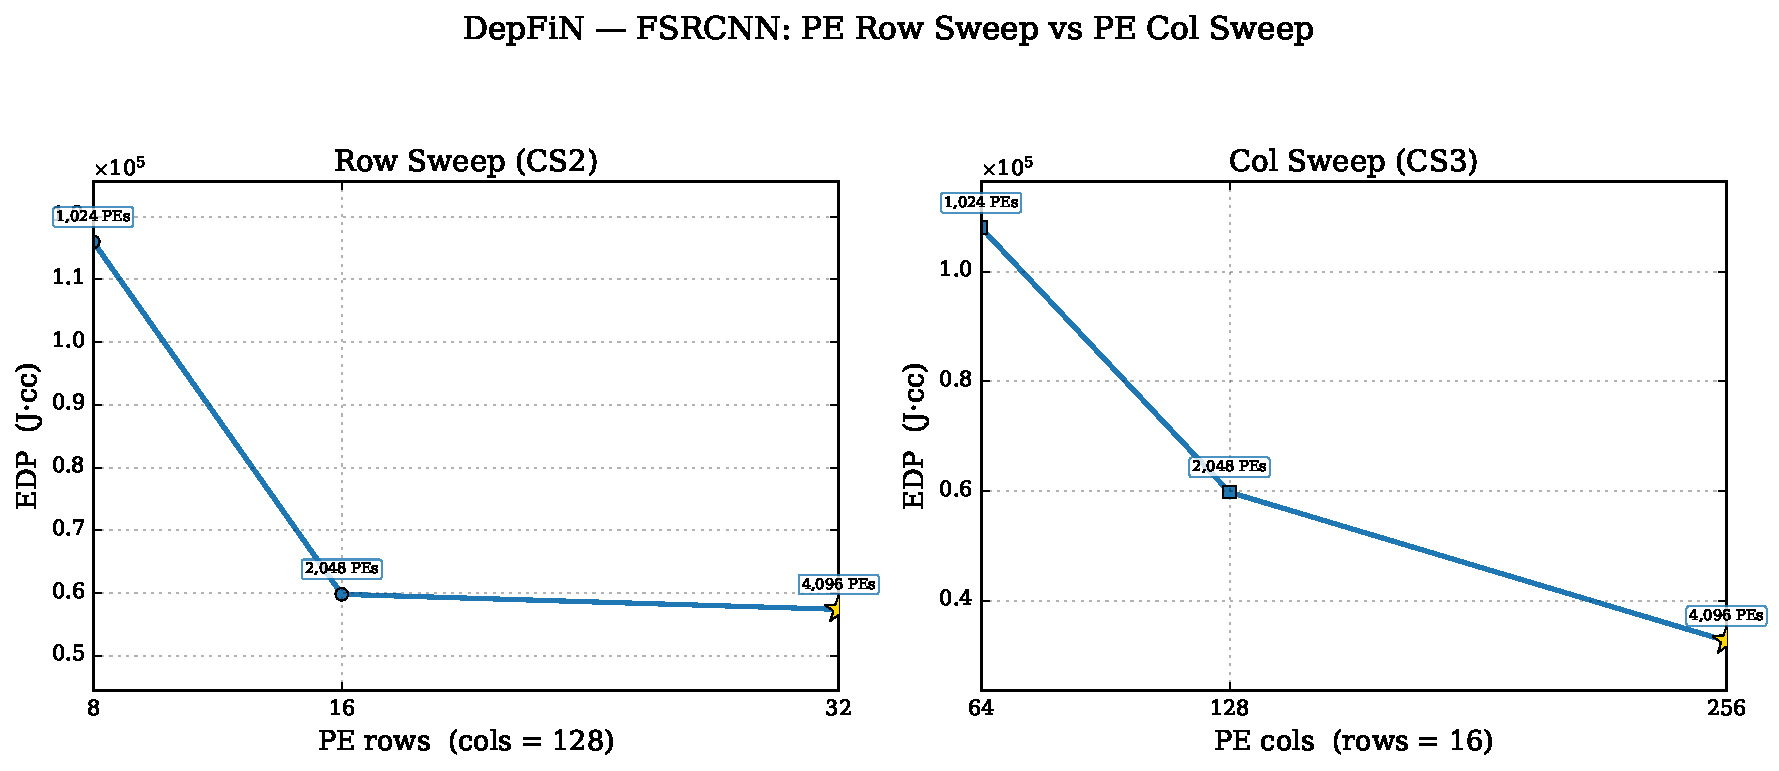
\includegraphics[width=0.85\textwidth]{plots/depfin_cs2cs3_fsrcnn.pdf}
  \caption{DepFiN CS2\,+\,CS3: FSRCNN: row sweep (left) and
    column sweep (right).}
  \label{fig:cs2cs3-fsrcnn}
\end{figure}

\begin{figure}[htbp]
  \centering
  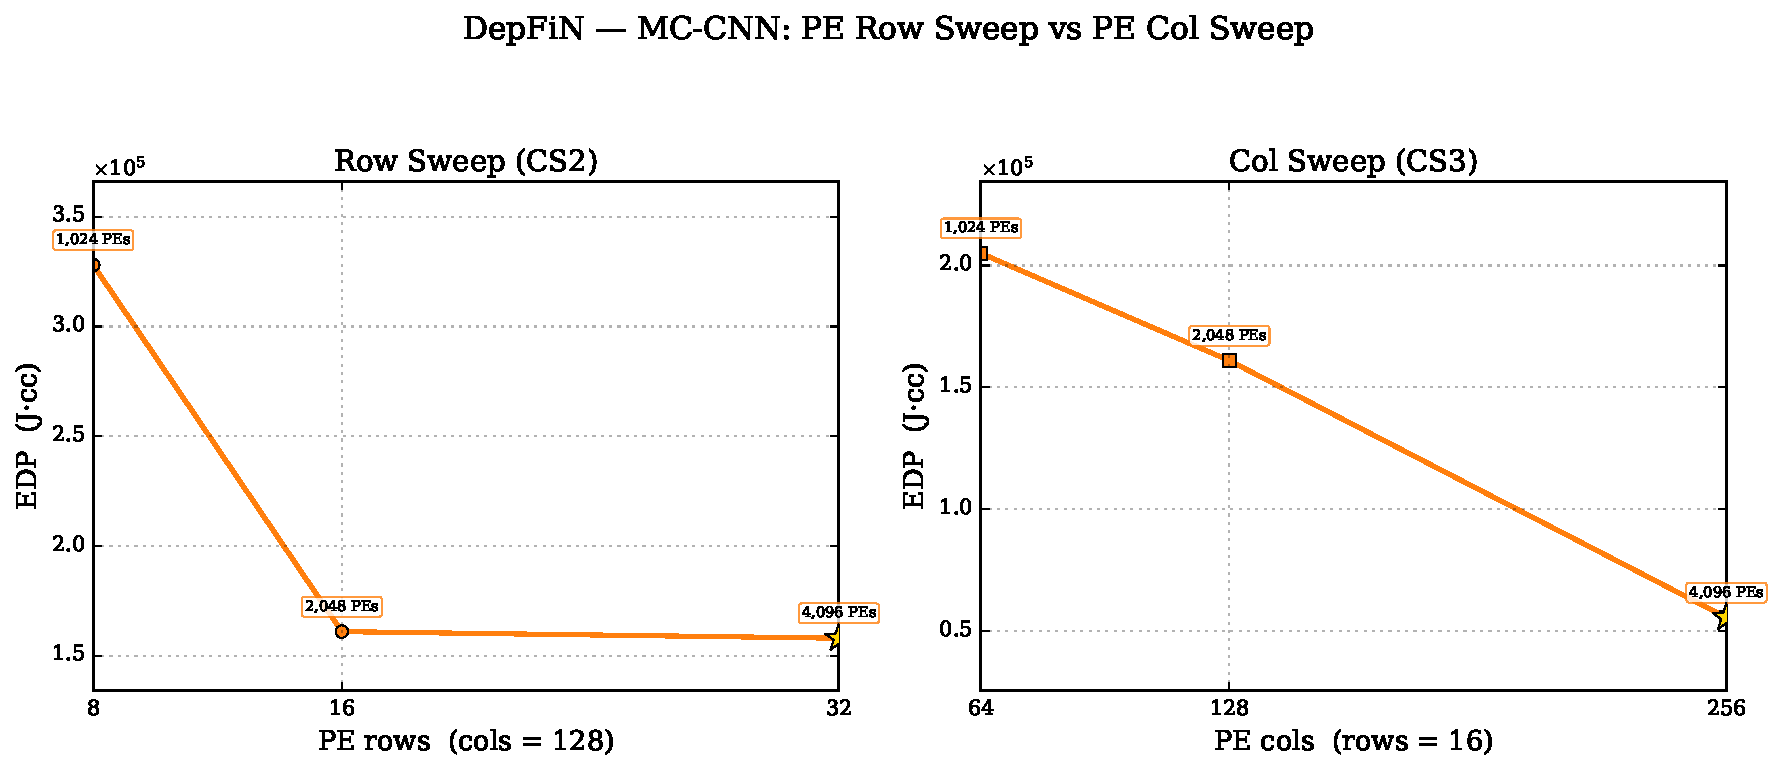
\includegraphics[width=0.85\textwidth]{plots/depfin_cs2cs3_mccnn.pdf}
  \caption{DepFiN CS2\,+\,CS3: MC-CNN: row sweep (left) and
    column sweep (right).}
  \label{fig:cs2cs3-mccnn}
\end{figure}

\begin{figure}[htbp]
  \centering
  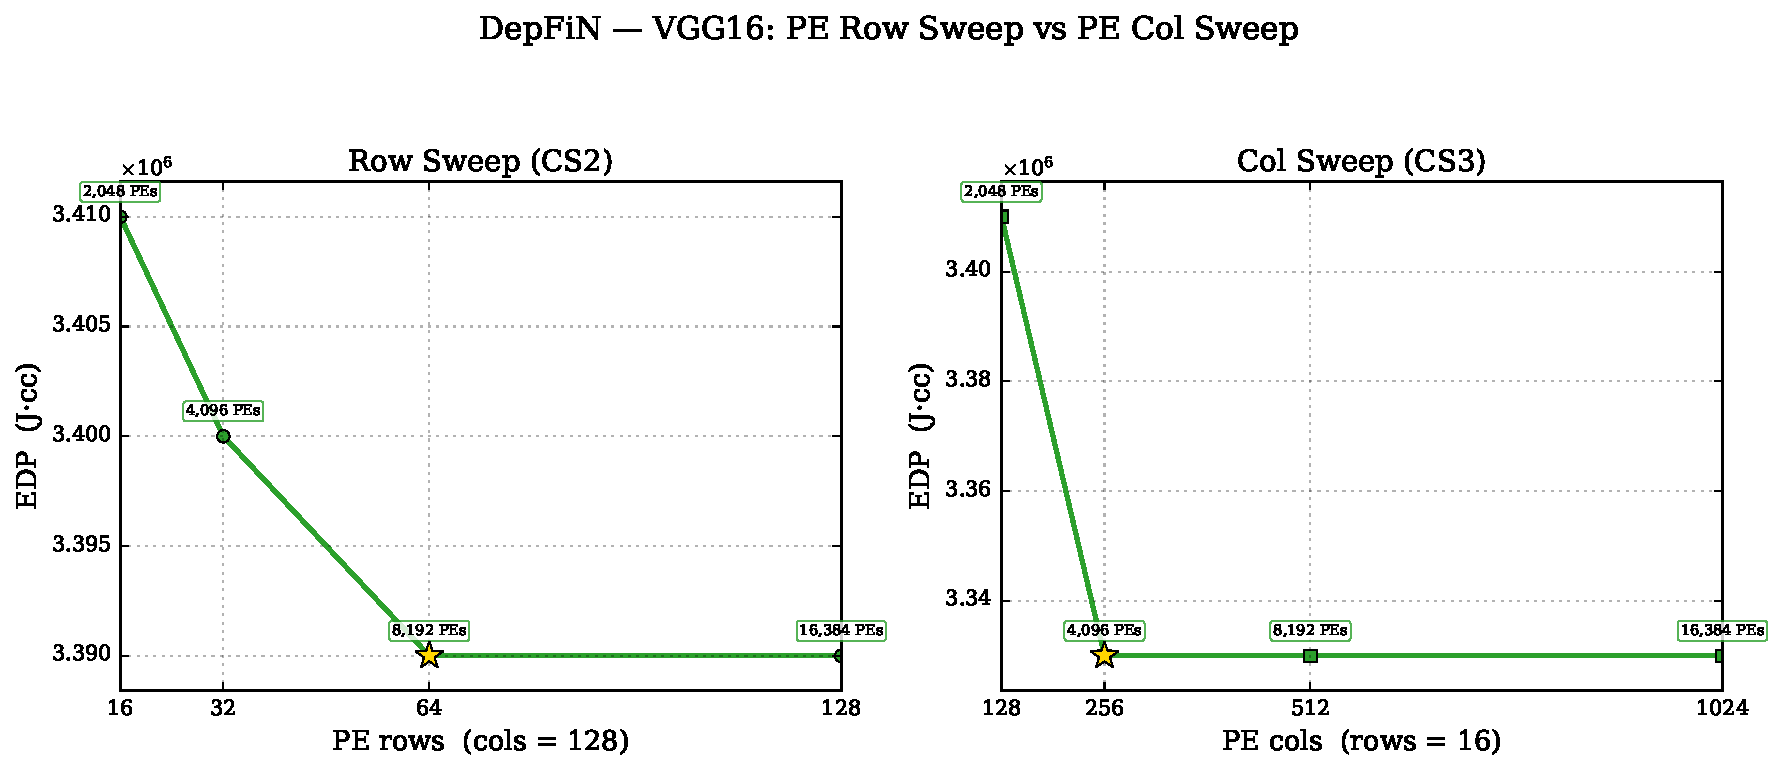
\includegraphics[width=0.85\textwidth]{plots/depfin_cs2cs3_vgg16.pdf}
  \caption{DepFiN CS2\,+\,CS3: VGG16: row sweep (left) and
    column sweep (right).}
  \label{fig:cs2cs3-vgg16}
\end{figure}

\begin{figure}[htbp]
  \centering
  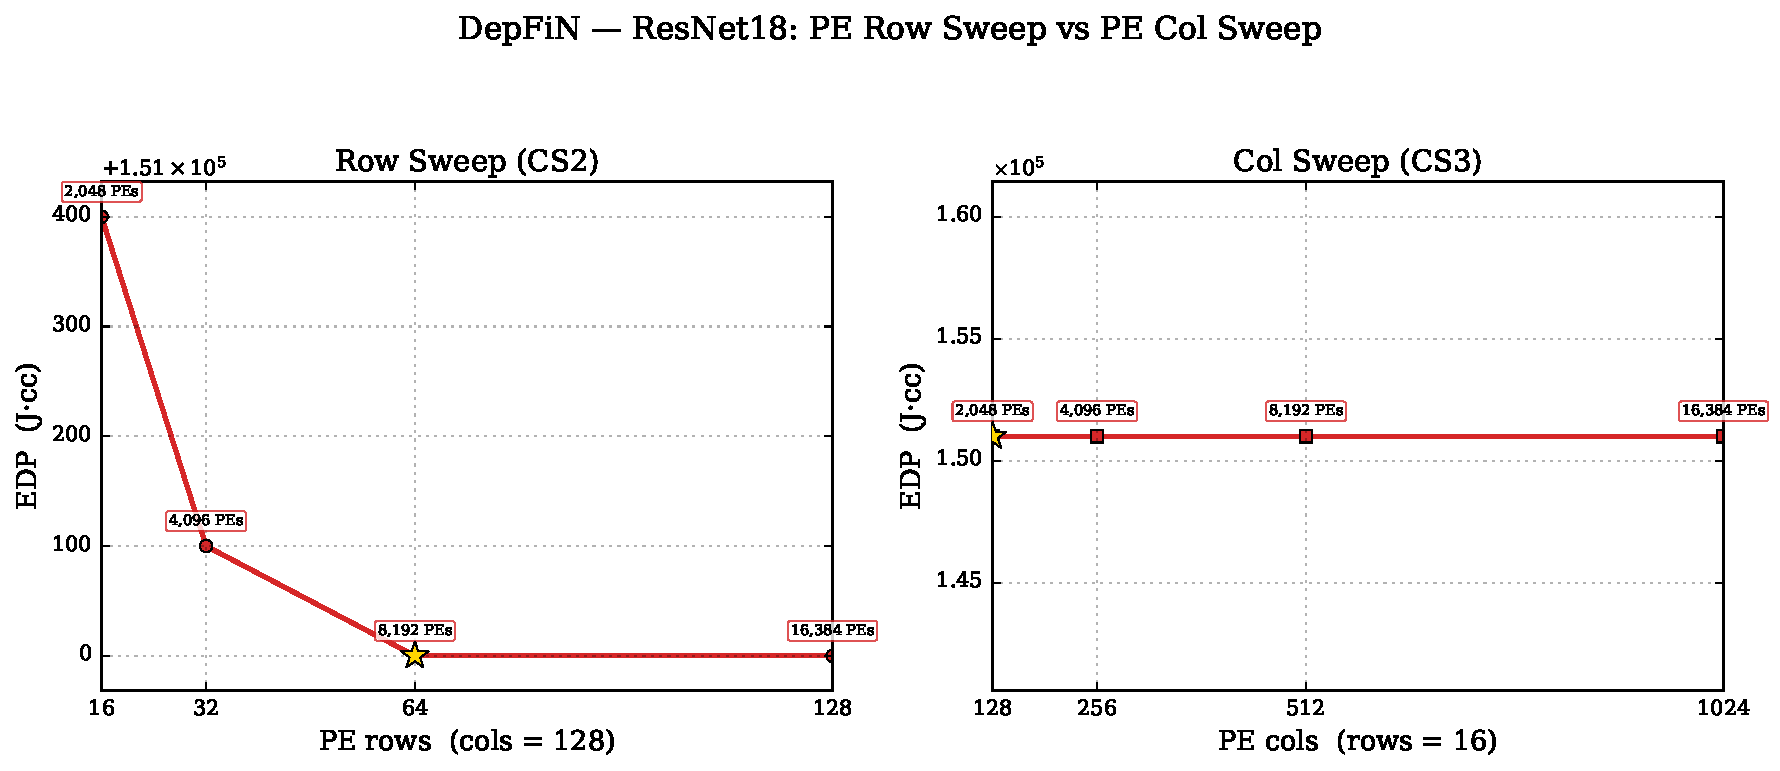
\includegraphics[width=0.85\textwidth]{plots/depfin_cs2cs3_resnet18.pdf}
  \caption{DepFiN CS2\,+\,CS3: ResNet18: row sweep (left) and
    column sweep (right).}
  \label{fig:cs2cs3-resnet18}
\end{figure}

\paragraph{Activation-dominant workloads (FSRCNN, MC-CNN).}
For these workloads the two dimensions produce markedly different
returns.
Taking FSRCNN as an example, the row sweep (CS2) reduces EDP by
$\approx 2\times$ going from 8 to 16 rows, but
doubling again to 32~rows yields only to a 4\% improvement.
The saturation occurs because, once the number of rows exceeds the
largest output-channel count in the fused group, the extra PE rows remain
idle.
In contrast, the column sweep (CS3) delivers a sustained reduction:
from 64 to 256 columns the EDP drops by $\approx 3.3\times$, with each doubling
roughly halving the EDP.
The benefit is sustained because adding columns enlarges the tile,
which directly reduces the number of DRAM-level passes and the
associated weight re-reads.

MC-CNN exhibits the same contrast: the row sweep saturates after
$2\times$ improvement, while the column
sweep achieves a $3.7\times$ reduction.


\paragraph{Weight-dominant workloads (VGG16, ResNet18).}
The row and column sweeps affect these workloads differently.
In the row sweep~(CS2), VGG16 EDP decreases by approximately~$9$\,\%
from 16 to 128~rows, driven entirely by a latency reduction as energy remains
essentially flat ($< 1$\,\% variation).
ResNet18 exhibits a similar pattern, with EDP decreasing by
approximately~$11$\,\%
Both workloads reach diminishing returns at 64~rows, beyond which
additional row parallelism provides no further benefit.
The latency improvement arises because, at fewer rows, DRAM
is the throughput bottleneck; adding rows relieves the DRAM-level
output-channel iterations, shifting the bottleneck to the Weight Memory.

In the column sweep~(CS3), both VGG16 and ResNet18 show
zero variation across all tested column configurations.
The spatial dimensions of both workloads already fit within
128~columns, so adding columns does not enlarge the tile or
reduce the DRAM pass count, the Spatial Fanout SACols is underutilized.

\paragraph{Considerations}
For activation-dominant workloads, additional PEs in columns
is substantially more effective than investing them in rows, because
columns enlarge the tile and reduce DRAM-level iterations, whereas
rows only reduce output-channel iterations, which saturate quickly.
For weight-dominant workloads, the row sweep provides a modest
latency-driven EDP improvement (${\sim}10$\,\%) by relieving the
DRAM bottleneck, but column scaling yields no benefit, as
the tile already spans the full spatial width at 128~columns.
Above 64~rows, performance is governed by the Weight Memory
bandwidth rather than by spatial parallelism.